\documentclass[final,5p]{elsarticle}
\ifdefined\pdfobjcompresslevel
  \pdfobjcompresslevel=0
\fi
\usepackage{amsmath,amssymb,amsfonts}
\usepackage{microtype,pifont}
\usepackage{graphicx}
\usepackage{dblfloatfix}
\usepackage[dvipsnames]{xcolor}
\usepackage{pgfplots}
\usepgfplotslibrary{groupplots}
\pgfplotsset{compat=1.18}
\usepackage{booktabs,multirow,tabularx,array,makecell}
\usepackage{algorithm,algorithmicx,algpseudocode}
\usepackage{enumitem, float,placeins}
\usepackage{caption}
\usepackage[colorlinks,bookmarksopen,bookmarksnumbered,citecolor=black, colorlinks=true,linkcolor=black,urlcolor=black,breaklinks=true]{hyperref}
\usepackage{xurl}
\usepackage{orcidlink}
\usepackage{balance}
% Permit top/bottom placement of two-column floats and reduce float starvation.
\setcounter{topnumber}{3}
\setcounter{dbltopnumber}{3}
\renewcommand{\topfraction}{0.9}
\renewcommand{\dbltopfraction}{0.9}
\renewcommand{\bottomfraction}{0.8}
\renewcommand{\textfraction}{0.05}
\renewcommand{\floatpagefraction}{0.75}
\renewcommand{\dblfloatpagefraction}{0.75}

% =========================
% Commands and styles
% =========================
\newcommand{\cmark}{\textcolor{ForestGreen}{\ding{51}}}
\newcommand{\xmark}{\textcolor{BrickRed}{\ding{55}}}
\ifdefined\CleanRevision
  \colorlet{revisiongreen}{black}
\else
  \colorlet{revisiongreen}{ForestGreen}
\fi
\newcommand{\rev}[1]{\textcolor{revisiongreen}{#1}}
\let\newrev\rev
% Use TeX primitive input for row fragments immediately before booktabs rules.
\newcommand{\TableRows}[1]{\csname @@input\endcsname{#1}}

\newcolumntype{R}[1]{>{\raggedleft\arraybackslash}m{#1}}
\newcolumntype{L}[1]{>{\raggedright\arraybackslash}m{#1}}
\newcolumntype{C}[1]{>{\centering\arraybackslash}m{#1}}

\renewcommand{\algorithmicrequire}{\textbf{Input:}}
\renewcommand{\algorithmicensure}{\textbf{Output:}}
\algrenewcommand\algorithmiccomment[1]{\hfill{\footnotesize$\triangleright$ #1}}

\makeatletter
\newcommand{\algorithmautorefname}{Algorithm}
\renewcommand{\figureautorefname}{Figure}
\renewcommand{\tableautorefname}{Table}
\renewcommand{\equationautorefname}{Eq.}
\renewcommand{\sectionautorefname}{Section}
\makeatother

\journal{Future Generation Computer Systems}

% Generated by scripts/paper/make_numbers.py.
\newcommand{\HILRequests}{12,325}
\newcommand{\SweepPeakGain}{2.58--3.80}
\newcommand{\SweepFinalGain}{2.41--3.31}

% Generated by scripts/paper/make_hil_e2e.py.
\newcommand{\HILEtoEOffered}{398}
\newcommand{\HILEtoESteered}{69}
\newcommand{\HILEtoEFullProbes}{64}
\newcommand{\HILEtoESubmitSteerPNF}{31.6}
\newcommand{\HILEtoESubmitSteerPF}{23.2}
\newcommand{\HILEtoEMigrations}{57}
\newcommand{\HILEtoEReprobeOK}{4}
\newcommand{\HILEtoEReprobeN}{4}
\newcommand{\HILLongPackets}{1,800}
\newcommand{\HILLongRecv}{1,800}
\newcommand{\HILLongRequests}{3,084}

\newcommand{\TrainingMeanMin}{57.375}
\newcommand{\TrainingMeanMax}{57.657}
\newcommand{\TrainingMeanSD}{0.156}

\begin{document}
\title{AIO-Mesh: Supplementary Results}
\author{Hanh P. Du et al.}
\maketitle
\setcounter{table}{0}
\renewcommand{\thetable}{S\arabic{table}}
\renewcommand{\theHtable}{supplement.\arabic{table}}
\begin{table*}[t]
\centering
\caption{Positioning of AIO-Mesh against representative related work. \rev{The MSD column concerns explicit SRv6 admission, not general resource-constraint handling.}}
\label{tab:related_comparison}
\renewcommand{\arraystretch}{1.15}
\resizebox{\textwidth}{!}{
\begin{tabular}{p{4.0cm}p{3.1cm}p{2.0cm}p{2.0cm}p{2.0cm}p{1.8cm}p{1.8cm}}
\toprule
\textbf{Work line} & \textbf{Primary focus} & \textbf{Cloud-native lifecycle} & \textbf{Graph-aware policy} & \rev{\textbf{SRv6 MSD admission}} & \textbf{Program- mable actuation} & \textbf{AIOps runtime} \\
\midrule
Classical ILP / greedy heuristics & SFC placement and routing & No & Limited & \rev{Varies} & No & No \\
DRL-based SFC placement~\cite{wang2021drl,taktak2024drl,li2023qosaware} & Online SFC embedding & No & Partial & No & No & No \\
\rev{Graph-assisted embedding}~\cite{xiao2023twostage,pei2025graph,liu2024sfcml} & Topology-aware embedding & No & Yes & No & No & No \\
SFC migration studies~\cite{zhai2023migration,addad2022ai,qin2023sfcmigrationbudget,afrasiabi2024cluster,zhang2025sfcmigration,hu2026rlpmo} & Load/failure migration & Partial & Varies & No & No & Limited \\
SRv6/P4 service-chain systems~\cite{stockmayer2020p4sfc,xiang2019p4sc,yan2024srv6int,li2024stsfc,ma2024sfcache} & Programmable steering & Limited & Partial & Partial & Yes & Limited \\
\newrev{Safe RL for network slicing~\cite{liu2021safeslicing,nagib2025safeslice}} & \newrev{Resource and latency constraints} & Partial & Varies & No & No & Limited \\
SFCPlanner~\cite{qiu2024sfcplanner} & SRv6-aware planning & No & Partial & Partial & Yes & No \\
AIOps/MLOps automation~\cite{kreuzberger2023mlops,diazdearcaya2024joint,eken2025mlops,bayram2025trustworthy,zhang2025aiopsllm,eramo2024architecture} & Operational ML loops & Partial & Not network-specific & No & No & Yes \\
\textbf{AIO-Mesh / HARP} & Hardware-safe AIOps orchestration & \textbf{Yes} & \textbf{Yes} & \rev{Pair-level} & \textbf{Yes} & \textbf{Yes} \\
\bottomrule
\end{tabular}
}
\end{table*}

\begin{table*}[t]
\centering
\caption{\newrev{Protocols supporting the simulation evaluation. All use 20 evaluation seeds and 3,000 simulator steps per seed and condition. Main-policy and ablation checkpoints are distinct.}}
\label{tab:evaluation_protocols}
\color{revisiongreen}
\scriptsize
\begin{tabular}{p{0.18\textwidth}p{0.19\textwidth}p{0.25\textwidth}p{0.28\textwidth}}
\toprule
Experiment & Checkpoint/interface & Offered traffic and occupancy & Interpretation \\
\midrule
Algorithm benchmark & Corrected main retrain, flat N² head & Three stress workloads; arrival 1.0; TTL 100--500 & Six topologies; completed seed-level results with 20 evaluation seeds per cell \\
Matched-trace ablation & Variant-specific flat-action policies & Four workloads; arrival 1.0; TTL 100--500 & Candidate quality, pruning, and modeled admission; distinct trained variants \\
Timed ablation & Variant-specific flat-action policies & Ten topology--workload conditions; arrival 1.0; TTL 100--500 & Simulator normalization, inference, and stepping; external actuation excluded \\
Background chains & Corrected main flat N² checkpoints & Bursty; arrival 1.0; 0/25/50/100 persistent chains; topology-scaled TTL & Completed occupancy sweep; 20 evaluation seeds per condition \\
Arrival-rate-only & Corrected main flat N² checkpoints & Bursty; arrival probability 0.2--1.0; fixed TTL 100--500 & Isolates arrival probability; 15 topology--rate cells and 20 matched evaluation seeds per policy \\
Load-sweep protocol & Corrected main flat N² checkpoints & Bursty at seven multipliers from 0.2 to 1.5; above 1.0, scale demand, requested SID depth, and TTL & Completed combined offered-intensity sweep; 21 topology--intensity cells and 20 evaluation seeds \\
\bottomrule
\end{tabular}
\end{table*}

\begin{table}[t]
\centering
\color{revisiongreen}
\caption{\newrev{Paired protected HARP--CSPF safe-acceptance differences (percentage points; 20 matched seeds). CIs are percentile-bootstrap 95\%; $p_H$ is the two-sided Wilcoxon $p$-value with Holm correction across nine conditions; $r$ is the paired rank-biserial effect.}}
\label{tab:cspf_paired_statistics}
\scriptsize
\setlength{\tabcolsep}{2.5pt}
\resizebox{\columnwidth}{!}{%
\begin{tabular}{llrrrr}
\toprule
Network & Profile & $\Delta$ & 95\% CI & $p_H$ & $r$ \\
\midrule
Vietnam & E & 0.392 & [0.215, 0.577] & 0.00142 & 0.810 \\
Vietnam & B & 0.872 & [0.603, 1.130] & 0.000187 & 0.943 \\
Vietnam & C & 0.650 & [0.477, 0.828] & 0.000787 & 1.000 \\
NSFNET & E & 0.672 & [0.487, 0.867] & 4.58e-05 & 0.981 \\
NSFNET & B & 0.742 & [0.560, 0.932] & 1.72e-05 & 1.000 \\
NSFNET & C & 0.902 & [0.655, 1.143] & 0.000787 & 0.989 \\
GEANT2 & E & 0.518 & [0.305, 0.718] & 0.00105 & 0.857 \\
GEANT2 & B & 0.183 & [0.045, 0.328] & 0.0759 & 0.462 \\
GEANT2 & C & 0.623 & [0.425, 0.832] & 0.00105 & 0.947 \\
\bottomrule
\end{tabular}%
}
\end{table}

\begin{table}[t]
\centering
\caption{\newrev{Full-policy safe acceptance and decision timing (20 seeds; mean $\pm$ sample SD). Timing summarizes seed-level P95 values; it is not a pooled request-level P95.}}
\label{tab:timed_full_coverage}
{\color{revisiongreen}\scriptsize
\setlength{\tabcolsep}{3pt}
\resizebox{\columnwidth}{!}{%
\begin{tabular}{llrr}
\toprule
Network & Workload & Safe (\%) & P95 (ms) \\
\midrule
GEANT2 & Bursty & 80.52 $\pm$ 0.46 & 2.969 $\pm$ 0.032 \\
GEANT2 & Uniform & 71.32 $\pm$ 0.36 & 2.802 $\pm$ 0.079 \\
NSFNET & Bursty & 66.83 $\pm$ 0.56 & 2.242 $\pm$ 0.051 \\
NSFNET & Chaos & 52.34 $\pm$ 0.73 & 2.223 $\pm$ 0.063 \\
NSFNET & Heavy-tail & 51.43 $\pm$ 0.54 & 2.187 $\pm$ 0.055 \\
NSFNET & Uniform & 56.81 $\pm$ 0.69 & 2.173 $\pm$ 0.025 \\
Vietnam & Bursty & 56.83 $\pm$ 0.78 & 2.250 $\pm$ 0.062 \\
Vietnam & Chaos & 43.31 $\pm$ 0.84 & 1.986 $\pm$ 0.031 \\
Vietnam & Heavy-tail & 42.79 $\pm$ 0.70 & 2.105 $\pm$ 0.145 \\
Vietnam & Uniform & 47.10 $\pm$ 0.54 & 2.201 $\pm$ 0.111 \\
\bottomrule
\end{tabular}%
}}
\end{table}

\begin{table*}[t]
\centering
\caption{Candidate pruning and local admission outcomes under matched traces (20 evaluation seeds across four workloads; mean $\pm$ sample SD over 80 seed--workload cells per topology, percentages). Empty-mask and conditional pruning columns report means.}
\label{tab:mask_admission}
\scriptsize
\begin{tabular}{llrrrrr}
\toprule
Topology & Variant & All pruning & Empty mask & Pruning if nonempty & Admitted violations & Safe acceptance \\
\midrule
\TableRows{generated/table09_rows.tex}
\bottomrule
\end{tabular}
\end{table*}

\begin{table*}[t]
\centering
\caption{\newrev{Control-plane HIL summary. Counts and percent denominators are derived from the request log; readiness counts use the 60-second Kubernetes samples.}}
\label{tab:hil_12h}
{\color{revisiongreen}
\small
% Generated by scripts/paper/make_table11.py; do not hand-edit.
\begin{tabular}{@{}lr@{}}
\toprule
Metric & Observed value \\
\midrule
API requests & 12,325 \\
Requested SID depth 1 / 2 & 4,964 / 7,361 \\
Configured per-node MSD limit (SID entries) & 10.0, 10.0, 5.0, 5.0, 4.0, 8.0, 4.0, 5.0, 10.0, 5.0 \\
Admitted (HTTP 200) & 1,455 (11.81\%) \\
Rejected (HTTP 409) & 10,870 (88.19\%) \\
\quad MSD rejection & 9,672 (78.47\%) \\
\quad Other no-safe-action & 1,198 (9.72\%) \\
\quad CPU/RAM capacity rejection & 0 (0.00\%) \\
API timeouts & 0 \\
Accepted policy / branch & Hybrid:DRL / drl \\
Client-observed API RTT P50 / P95 / P99 (ms) & 118.19 / 169.95 / 229.40 \\
Hourly API RTT P95 range (ms) & 164.60--175.30 \\
Hourly admission-rate range (\% of requests) & 9.44--13.92 \\
Backend policy inference P50 / P95 / P99 (ms; admitted only) & 74.89 / 117.73 / 154.42 \\
Backend admission validation P50 / P95 / P99 (ms; admitted only) & 18.28 / 29.47 / 41.53 \\
Actuation requested / deployment confirmed & 0 / 0 \\
Baseline Deployments Ready & 7/7 in 720/720 samples \\
Baseline replicas Ready & 7/7 in 720/720 samples \\
MSD drops / forwarding & not measured / not part of this run \\
\bottomrule
\end{tabular}

}
\end{table*}

\begin{table}[t]
\centering
\caption{\newrev{Protected-policy safe acceptance across the load sweep (\%; mean $\pm$ sample SD, 20 seeds). Load denotes offered intensity; DAI denotes Decoupled AI.}}
\label{tab:load_sweep_results}
\scriptsize
{\color{revisiongreen}
\setlength{\tabcolsep}{3pt}
\resizebox{\columnwidth}{!}{%
\begin{tabular}{llrrrrr}
\toprule
Network & Load & Greedy & DAI & SAF-H & CSPF & HARP \\
\midrule
\TableRows{evidence/completion_20261121/load_cspf.tex}
\bottomrule
\end{tabular}%
}}
\end{table}

\begin{table*}[t]
\centering
\caption{\newrev{Sampled exhaustive pair-action oracle on Vietnam (10 seeds; 120 states per seed). Conditional rates are seed-level means with sample SD.}}
\label{tab:missed_feasible_oracle}
\scriptsize
{\color{revisiongreen}
\setlength{\tabcolsep}{3pt}
\resizebox{\textwidth}{!}{%
\begin{tabular}{lrrrr}
\toprule
Policy & Sampled states & Selected rejections & With accepted alternative & Conditional rate (\%; mean $\pm$ SD) \\
\midrule
HARP & 1,200 & 583 & 30 & 5.16 $\pm$ 1.84 \\
SAF-H & 1,200 & 579 & 33 & 5.70 $\pm$ 2.32 \\
\bottomrule
\end{tabular}%
}}
\end{table*}

\begin{table}[t]
\centering
\caption{Safe acceptance under long-lived background-chain occupancy (20 seeds; mean $\pm$ sample SD, percentages).}
\label{tab:active_chain_stress}
\scriptsize
\setlength{\tabcolsep}{3pt}
\resizebox{\columnwidth}{!}{%
\begin{tabular}{lrrrr}
\toprule
Network & Chains & HARP & SAF-H & CSPF \\
\midrule
\TableRows{evidence/completion_20261121/chains_cspf.tex}
\bottomrule
\end{tabular}%
}
\end{table}

\begin{table*}[t]
\centering
\caption{Protected safe acceptance on synthetic topologies (percent; mean $\pm$ sample SD across 20 seeds). E, B, and C denote Elephant stress, Burst surge, and Chaos.}
\label{tab:synthetic_stress}
\scriptsize
\begin{tabular}{llrrrrr}
\toprule
Nodes & Profile & Greedy & DAI & SAF-H & CSPF & HARP \\
\midrule
\TableRows{evidence/model_refresh_20261120/synthetic_stress_table_rows.tex}
\bottomrule
\end{tabular}
\end{table*}

\begin{table*}[t]
\centering
\caption{Exploratory HARP minus strongest protected baseline safe acceptance (percentage points; 20 paired seeds). The strongest baseline is selected by sample mean in the same cell. $p_H$ uses Holm correction over nine real-topology comparisons; selection uncertainty is not accounted for.}
\label{tab:best_baseline_exploratory}
\scriptsize
\begin{tabular}{lllrrrr}
\toprule
Network & Profile & Baseline & $\Delta$ & 95\% CI & $p_H$ & $n_{eff}$ \\
\midrule
\TableRows{evidence/completion_20261121/best_baseline.tex}
\bottomrule
\end{tabular}
\end{table*}

\begin{table}[t]
\centering
\caption{Pre-step mask and admission audit: 20 seeds and 60,000 decisions per topology. Last column counts empty masks becoming nonempty after pending TTL expiry.}
\label{tab:mask_ttl_audit}
\scriptsize
\resizebox{\columnwidth}{!}{%
\begin{tabular}{lrrrr}
\toprule
Network & Empty & Rejected, empty & Rejected, nonempty & Empty $\rightarrow$ nonempty \\
\midrule
\TableRows{evidence/mentor_completion_20261121/mask_table.tex}
\bottomrule
\end{tabular}}
\end{table}

\begin{table}[t]
\centering
\caption{Full GAT versus MLP under synthetic sparse adjacency (20 matched Bursty seeds; safe acceptance percent, paired difference in percentage points with 95\% bootstrap CI).}
\label{tab:sparse_gat_mlp}
\scriptsize
\resizebox{\columnwidth}{!}{%
\begin{tabular}{lrrrr}
\toprule
Network & Full & MLP & Difference & 95\% CI \\
\midrule
\TableRows{evidence/mentor_completion_20261121/sparse_table.tex}
\bottomrule
\end{tabular}}
\end{table}

\begin{table}[t]
\centering
\caption{Sampled pair oracle for the offered-intensity protocol. Counts aggregate ten seeds; sampled states are not independent replications.}
\label{tab:oracle_load_followup}
\scriptsize
\resizebox{\columnwidth}{!}{%
\begin{tabular}{llrrrr}
\toprule
Network & Load & Policy & States & Rejected & With alternative \\
\midrule
\TableRows{evidence/mentor_completion_20261121/oracle_table.tex}
\bottomrule
\end{tabular}}
\end{table}
\section*{Supplementary Results}
\begingroup
\setcounter{figure}{0}
\renewcommand{\thefigure}{S\arabic{figure}}
\renewcommand{\theHfigure}{supplement.\arabic{figure}}
\renewcommand{\thetable}{S\arabic{table}}
\renewcommand{\theHtable}{supplement.\arabic{table}}
\begin{figure*}[p]
\centering
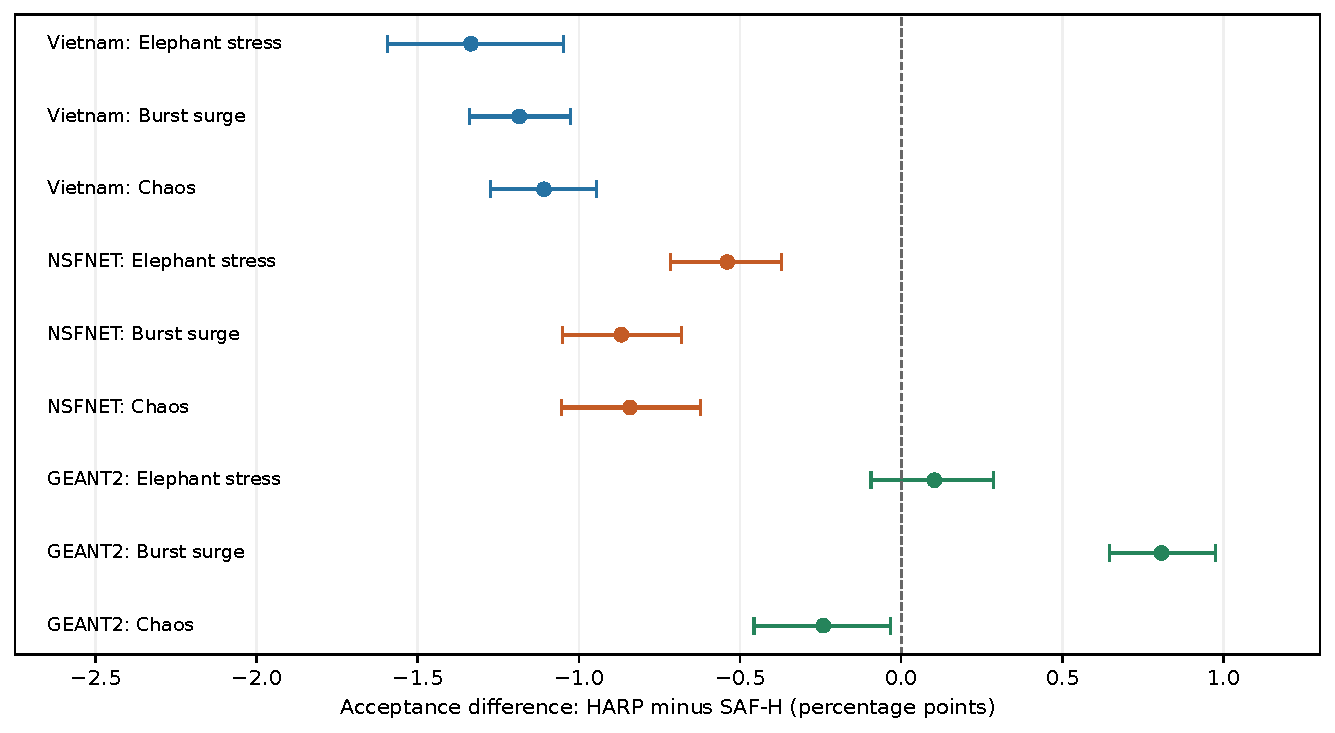
\includegraphics[width=0.94\textwidth]{figs/benchmark_paired_effects.pdf}
\caption{\newrev{Protected HARP minus SAF-H acceptance across three topologies and three stress workloads. Points show mean paired seed-level differences; horizontal intervals are percentile-bootstrap 95\% confidence intervals from paired seed-level trials. Positive values favor HARP. Holm-adjusted tests across all nine conditions are reported in Table~3.}}
\label{fig:benchmark_effects}
\end{figure*}

\begin{figure*}[p]
\centering
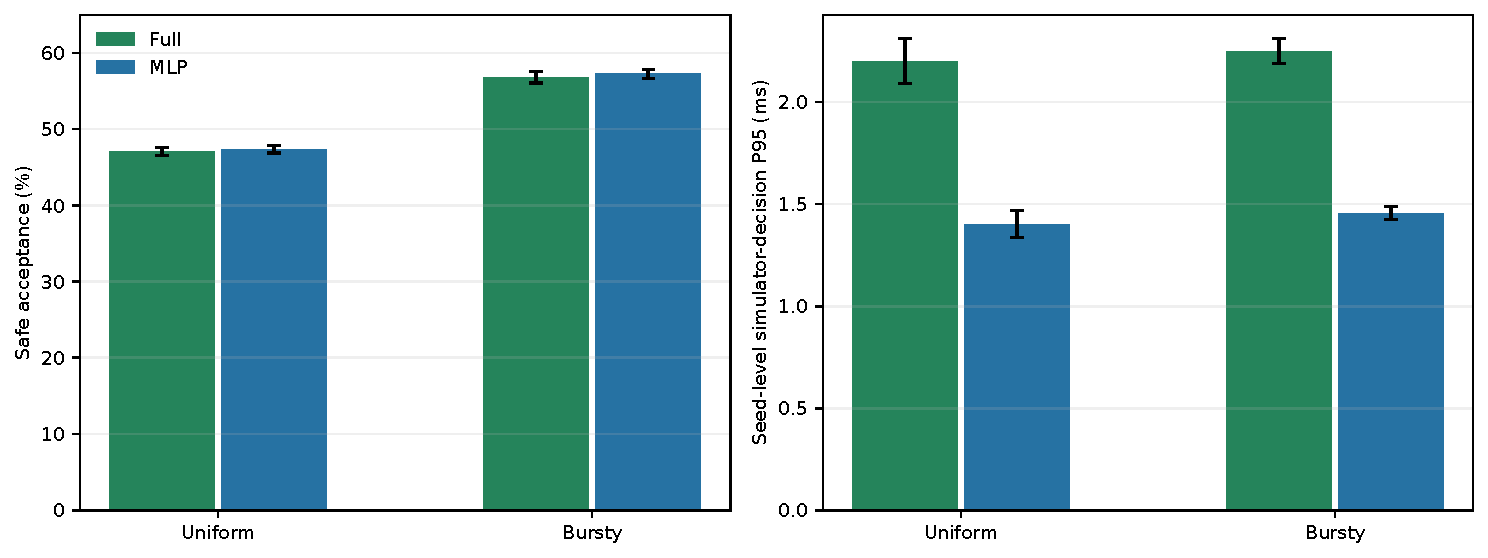
\includegraphics[width=0.94\textwidth]{figs/ablation_compute_cost.pdf}
\caption{\newrev{Acceptance and measured computation cost of Full and MLP ablation checkpoints on Vietnam. Bars show means and error bars show sample SD across 20 evaluation seeds. The right panel aggregates the per-seed P95 interval including normalization, inference, and simulator stepping; it excludes external controller actuation.}}
\label{fig:ablation_cost}
\end{figure*}

\begin{figure*}[p]
\centering
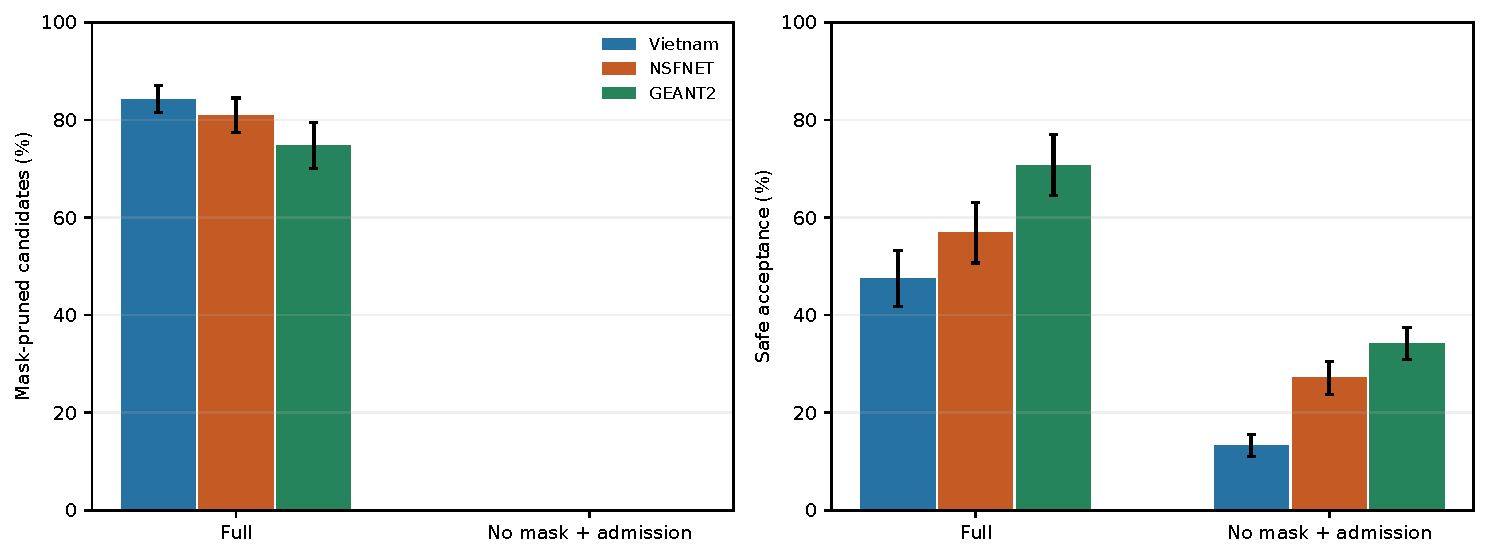
\includegraphics[width=0.94\textwidth]{figs/ablation_mask_admission.pdf}
\caption{\newrev{Candidate pruning and safe acceptance for Full and NoMask ablation variants with runtime admission enabled. Bars summarize 80 seed--workload cells per topology; error bars are sample SD across those cells. All six protected configurations recorded zero admitted hard violations. Distinct checkpoints and resulting state trajectories limit causal attribution to masking alone.}}
\label{fig:ablation_pruning}
\end{figure*}

\begin{table*}[p]
\centering
\color{revisiongreen}\small
\begin{tabular}{llrrrrrr}
\toprule
Topology & Intensity & $\Delta$ (pp) & 95\% CI & $p$ & $r_{rb}$ & $n_{eff}$ & $p_{\mathrm{Holm}}$ \\
\midrule
VIETNAM & 0.2 & 0.000 & [0.000, 0.000] & 1 & -- & 0 & 1 \\
VIETNAM & 0.4 & 0.004 & [0.000, 0.012] & 1 & 1.000 & 1 & 1 \\
VIETNAM & 0.6 & 0.019 & [0.006, 0.038] & 0.0625 & 1.000 & 5 & 0.562 \\
VIETNAM & 0.8 & 0.403 & [0.351, 0.454] & 1.91e-06 & 1.000 & 20 & 4.01e-05 \\
VIETNAM & 1.0 & 1.160 & [1.078, 1.240] & 1.91e-06 & 1.000 & 20 & 4.01e-05 \\
VIETNAM & 1.2 & 2.577 & [2.483, 2.668] & 1.91e-06 & 1.000 & 20 & 4.01e-05 \\
VIETNAM & 1.5 & 2.408 & [2.308, 2.512] & 1.91e-06 & 1.000 & 20 & 4.01e-05 \\
NSFNET & 0.2 & 0.000 & [0.000, 0.000] & 1 & -- & 0 & 1 \\
NSFNET & 0.4 & 0.000 & [0.000, 0.000] & 1 & -- & 0 & 1 \\
NSFNET & 0.6 & 0.014 & [0.003, 0.028] & 0.125 & 1.000 & 4 & 1 \\
NSFNET & 0.8 & 0.249 & [0.197, 0.304] & 1.91e-06 & 1.000 & 20 & 4.01e-05 \\
NSFNET & 1.0 & 1.127 & [1.067, 1.185] & 1.91e-06 & 1.000 & 20 & 4.01e-05 \\
NSFNET & 1.2 & 3.158 & [3.000, 3.310] & 1.91e-06 & 1.000 & 20 & 4.01e-05 \\
NSFNET & 1.5 & 2.757 & [2.665, 2.848] & 1.91e-06 & 1.000 & 20 & 4.01e-05 \\
GEANT2 & 0.2 & 0.000 & [0.000, 0.000] & 1 & -- & 0 & 1 \\
GEANT2 & 0.4 & 0.000 & [0.000, 0.000] & 1 & -- & 0 & 1 \\
GEANT2 & 0.6 & 0.006 & [0.000, 0.014] & 0.5 & 1.000 & 2 & 1 \\
GEANT2 & 0.8 & 0.120 & [0.089, 0.154] & 3.81e-06 & 1.000 & 19 & 4.01e-05 \\
GEANT2 & 1.0 & 0.985 & [0.928, 1.040] & 1.91e-06 & 1.000 & 20 & 4.01e-05 \\
GEANT2 & 1.2 & 3.803 & [3.688, 3.915] & 1.91e-06 & 1.000 & 20 & 4.01e-05 \\
GEANT2 & 1.5 & 3.312 & [3.208, 3.412] & 1.91e-06 & 1.000 & 20 & 4.01e-05 \\
\bottomrule
\end{tabular}
\caption{Paired HARP--SAF-H safe-acceptance differences in the load sweep. $\Delta$ is the mean over matched seeds; CI is the 20,000-resample paired percentile-bootstrap 95\% interval. $p$ is the exact two-sided Wilcoxon signed-rank p-value with zero differences dropped and tied absolute ranks averaged. All-zero comparisons use $p_H=1$, $n_{eff}=0$, and undefined $r_{rb}$, and remain in the 21-test Holm family.}
\label{tab:load_sweep_paired_statistics}
\end{table*}

\begin{table*}[p]
\centering
\color{revisiongreen}\small
\begin{tabular}{llrrrrr}
\toprule
Intensity & Policy & CPU & RAM & BW & MSD & Any hard violation \\
\midrule
0.2 & Greedy & 0.000 $\pm$ 0.000 & 0.000 $\pm$ 0.000 & 0.000 $\pm$ 0.000 & 0.378 $\pm$ 0.201 & 0.378 $\pm$ 0.201 \\
0.2 & DAI & 0.000 $\pm$ 0.000 & 0.000 $\pm$ 0.000 & 0.000 $\pm$ 0.000 & 0.748 $\pm$ 0.310 & 0.748 $\pm$ 0.310 \\
0.2 & SAF-H & 0.000 $\pm$ 0.000 & 0.000 $\pm$ 0.000 & 0.000 $\pm$ 0.000 & 0.865 $\pm$ 0.334 & 0.865 $\pm$ 0.334 \\
0.2 & HARP & 5.224 $\pm$ 1.035 & 0.526 $\pm$ 0.356 & 0.000 $\pm$ 0.000 & 0.008 $\pm$ 0.037 & 5.233 $\pm$ 1.029 \\
0.4 & Greedy & 0.004 $\pm$ 0.018 & 0.000 $\pm$ 0.000 & 0.000 $\pm$ 0.000 & 0.368 $\pm$ 0.139 & 0.372 $\pm$ 0.134 \\
0.4 & DAI & 0.004 $\pm$ 0.018 & 0.000 $\pm$ 0.000 & 0.000 $\pm$ 0.000 & 0.687 $\pm$ 0.198 & 0.692 $\pm$ 0.201 \\
0.4 & SAF-H & 0.004 $\pm$ 0.018 & 0.000 $\pm$ 0.000 & 0.000 $\pm$ 0.000 & 0.728 $\pm$ 0.208 & 0.732 $\pm$ 0.210 \\
0.4 & HARP & 14.636 $\pm$ 1.346 & 3.702 $\pm$ 1.164 & 0.000 $\pm$ 0.000 & 0.151 $\pm$ 0.114 & 14.674 $\pm$ 1.356 \\
0.6 & Greedy & 0.019 $\pm$ 0.037 & 0.000 $\pm$ 0.000 & 0.000 $\pm$ 0.000 & 0.289 $\pm$ 0.154 & 0.308 $\pm$ 0.170 \\
0.6 & DAI & 0.019 $\pm$ 0.037 & 0.000 $\pm$ 0.000 & 0.000 $\pm$ 0.000 & 0.698 $\pm$ 0.153 & 0.715 $\pm$ 0.158 \\
0.6 & SAF-H & 0.019 $\pm$ 0.037 & 0.000 $\pm$ 0.000 & 0.000 $\pm$ 0.000 & 0.703 $\pm$ 0.176 & 0.720 $\pm$ 0.186 \\
0.6 & HARP & 30.797 $\pm$ 1.295 & 15.403 $\pm$ 1.721 & 0.000 $\pm$ 0.000 & 0.392 $\pm$ 0.091 & 30.903 $\pm$ 1.299 \\
0.8 & Greedy & 0.508 $\pm$ 0.152 & 0.002 $\pm$ 0.009 & 0.000 $\pm$ 0.000 & 0.351 $\pm$ 0.109 & 0.845 $\pm$ 0.185 \\
0.8 & DAI & 0.509 $\pm$ 0.150 & 0.000 $\pm$ 0.000 & 0.000 $\pm$ 0.000 & 0.735 $\pm$ 0.131 & 1.206 $\pm$ 0.188 \\
0.8 & SAF-H & 0.506 $\pm$ 0.146 & 0.000 $\pm$ 0.000 & 0.000 $\pm$ 0.000 & 0.756 $\pm$ 0.145 & 1.229 $\pm$ 0.235 \\
0.8 & HARP & 41.800 $\pm$ 1.405 & 29.837 $\pm$ 1.759 & 0.000 $\pm$ 0.000 & 0.497 $\pm$ 0.087 & 41.928 $\pm$ 1.399 \\
1.0 & Greedy & 2.158 $\pm$ 0.240 & 0.005 $\pm$ 0.012 & 0.000 $\pm$ 0.000 & 0.342 $\pm$ 0.113 & 2.467 $\pm$ 0.290 \\
1.0 & DAI & 2.158 $\pm$ 0.240 & 0.005 $\pm$ 0.012 & 0.000 $\pm$ 0.000 & 0.707 $\pm$ 0.150 & 2.765 $\pm$ 0.239 \\
1.0 & SAF-H & 2.162 $\pm$ 0.240 & 0.005 $\pm$ 0.012 & 0.000 $\pm$ 0.000 & 0.717 $\pm$ 0.114 & 2.775 $\pm$ 0.209 \\
1.0 & HARP & 46.428 $\pm$ 1.446 & 36.123 $\pm$ 1.551 & 0.000 $\pm$ 0.000 & 0.213 $\pm$ 0.070 & 46.472 $\pm$ 1.452 \\
1.2 & Greedy & 13.998 $\pm$ 0.688 & 0.557 $\pm$ 0.092 & 0.000 $\pm$ 0.000 & 0.345 $\pm$ 0.111 & 14.173 $\pm$ 0.702 \\
1.2 & DAI & 13.978 $\pm$ 0.777 & 0.660 $\pm$ 0.192 & 0.000 $\pm$ 0.000 & 0.722 $\pm$ 0.128 & 14.352 $\pm$ 0.755 \\
1.2 & SAF-H & 14.010 $\pm$ 0.669 & 0.555 $\pm$ 0.094 & 0.000 $\pm$ 0.000 & 0.638 $\pm$ 0.119 & 14.330 $\pm$ 0.660 \\
1.2 & HARP & 60.160 $\pm$ 1.564 & 45.993 $\pm$ 1.492 & 0.000 $\pm$ 0.000 & 0.020 $\pm$ 0.029 & 60.165 $\pm$ 1.567 \\
1.5 & Greedy & 58.993 $\pm$ 2.023 & 12.195 $\pm$ 0.790 & 0.000 $\pm$ 0.000 & 10.872 $\pm$ 0.309 & 60.855 $\pm$ 1.881 \\
1.5 & DAI & 47.770 $\pm$ 0.977 & 21.058 $\pm$ 0.786 & 0.000 $\pm$ 0.000 & 23.242 $\pm$ 0.808 & 53.555 $\pm$ 0.775 \\
1.5 & SAF-H & 58.972 $\pm$ 2.042 & 12.182 $\pm$ 0.774 & 0.000 $\pm$ 0.000 & 21.417 $\pm$ 0.205 & 62.790 $\pm$ 1.934 \\
1.5 & HARP & 70.958 $\pm$ 0.838 & 61.262 $\pm$ 0.915 & 0.083 $\pm$ 0.142 & 27.068 $\pm$ 0.262 & 72.905 $\pm$ 0.860 \\
\bottomrule
\end{tabular}
\caption{\newrev{Vietnam offered-intensity experiment with admission disabled. Rates are means and sample SD in percent over 20 seeds. The denominator is all offered requests. Constraint categories can overlap.}}
\label{tab:load_sweep_unprotected}
\end{table*}
\begin{table*}[p]
\centering
\color{revisiongreen}\small
\begin{tabular}{llrrrrr}
\toprule
Intensity & Policy & CPU & RAM & BW & MSD & Any hard violation \\
\midrule
0.2 & Greedy & 0.000 $\pm$ 0.000 & 0.000 $\pm$ 0.000 & 0.000 $\pm$ 0.000 & 0.000 $\pm$ 0.000 & 0.000 $\pm$ 0.000 \\
0.2 & DAI & 0.000 $\pm$ 0.000 & 0.000 $\pm$ 0.000 & 0.000 $\pm$ 0.000 & 0.000 $\pm$ 0.000 & 0.000 $\pm$ 0.000 \\
0.2 & SAF-H & 0.000 $\pm$ 0.000 & 0.000 $\pm$ 0.000 & 0.000 $\pm$ 0.000 & 0.000 $\pm$ 0.000 & 0.000 $\pm$ 0.000 \\
0.2 & HARP & 5.358 $\pm$ 1.162 & 0.060 $\pm$ 0.131 & 0.000 $\pm$ 0.000 & 0.000 $\pm$ 0.000 & 5.358 $\pm$ 1.162 \\
0.4 & Greedy & 0.000 $\pm$ 0.000 & 0.000 $\pm$ 0.000 & 0.000 $\pm$ 0.000 & 0.000 $\pm$ 0.000 & 0.000 $\pm$ 0.000 \\
0.4 & DAI & 0.000 $\pm$ 0.000 & 0.000 $\pm$ 0.000 & 0.000 $\pm$ 0.000 & 0.000 $\pm$ 0.000 & 0.000 $\pm$ 0.000 \\
0.4 & SAF-H & 0.000 $\pm$ 0.000 & 0.000 $\pm$ 0.000 & 0.000 $\pm$ 0.000 & 0.000 $\pm$ 0.000 & 0.000 $\pm$ 0.000 \\
0.4 & HARP & 12.539 $\pm$ 2.267 & 1.227 $\pm$ 0.623 & 0.000 $\pm$ 0.000 & 0.000 $\pm$ 0.000 & 12.539 $\pm$ 2.267 \\
0.6 & Greedy & 0.014 $\pm$ 0.040 & 0.000 $\pm$ 0.000 & 0.000 $\pm$ 0.000 & 0.000 $\pm$ 0.000 & 0.014 $\pm$ 0.040 \\
0.6 & DAI & 0.019 $\pm$ 0.045 & 0.000 $\pm$ 0.000 & 0.000 $\pm$ 0.000 & 0.000 $\pm$ 0.000 & 0.019 $\pm$ 0.045 \\
0.6 & SAF-H & 0.019 $\pm$ 0.045 & 0.000 $\pm$ 0.000 & 0.000 $\pm$ 0.000 & 0.000 $\pm$ 0.000 & 0.019 $\pm$ 0.045 \\
0.6 & HARP & 27.641 $\pm$ 1.744 & 5.884 $\pm$ 1.021 & 0.000 $\pm$ 0.000 & 0.000 $\pm$ 0.000 & 27.641 $\pm$ 1.744 \\
0.8 & Greedy & 0.330 $\pm$ 0.081 & 0.000 $\pm$ 0.000 & 0.000 $\pm$ 0.000 & 0.000 $\pm$ 0.000 & 0.330 $\pm$ 0.081 \\
0.8 & DAI & 0.332 $\pm$ 0.082 & 0.000 $\pm$ 0.000 & 0.000 $\pm$ 0.000 & 0.000 $\pm$ 0.000 & 0.332 $\pm$ 0.082 \\
0.8 & SAF-H & 0.330 $\pm$ 0.080 & 0.000 $\pm$ 0.000 & 0.000 $\pm$ 0.000 & 0.000 $\pm$ 0.000 & 0.330 $\pm$ 0.080 \\
0.8 & HARP & 47.571 $\pm$ 1.968 & 17.558 $\pm$ 1.500 & 0.000 $\pm$ 0.000 & 0.000 $\pm$ 0.000 & 47.577 $\pm$ 1.965 \\
1.0 & Greedy & 1.747 $\pm$ 0.203 & 0.005 $\pm$ 0.012 & 0.000 $\pm$ 0.000 & 0.000 $\pm$ 0.000 & 1.747 $\pm$ 0.203 \\
1.0 & DAI & 1.742 $\pm$ 0.201 & 0.005 $\pm$ 0.012 & 0.000 $\pm$ 0.000 & 0.000 $\pm$ 0.000 & 1.742 $\pm$ 0.201 \\
1.0 & SAF-H & 1.728 $\pm$ 0.206 & 0.005 $\pm$ 0.012 & 0.000 $\pm$ 0.000 & 0.000 $\pm$ 0.000 & 1.728 $\pm$ 0.206 \\
1.0 & HARP & 64.120 $\pm$ 2.055 & 32.200 $\pm$ 1.356 & 0.000 $\pm$ 0.000 & 0.000 $\pm$ 0.000 & 64.140 $\pm$ 2.046 \\
1.2 & Greedy & 12.332 $\pm$ 0.552 & 0.368 $\pm$ 0.091 & 0.000 $\pm$ 0.000 & 0.000 $\pm$ 0.000 & 12.332 $\pm$ 0.552 \\
1.2 & DAI & 12.307 $\pm$ 0.639 & 0.367 $\pm$ 0.079 & 0.000 $\pm$ 0.000 & 0.000 $\pm$ 0.000 & 12.307 $\pm$ 0.639 \\
1.2 & SAF-H & 12.288 $\pm$ 0.627 & 0.365 $\pm$ 0.097 & 0.000 $\pm$ 0.000 & 0.000 $\pm$ 0.000 & 12.288 $\pm$ 0.627 \\
1.2 & HARP & 79.660 $\pm$ 0.988 & 51.352 $\pm$ 1.307 & 0.000 $\pm$ 0.000 & 0.000 $\pm$ 0.000 & 79.665 $\pm$ 0.984 \\
1.5 & Greedy & 58.308 $\pm$ 2.128 & 11.053 $\pm$ 0.800 & 0.000 $\pm$ 0.000 & 1.008 $\pm$ 0.138 & 58.467 $\pm$ 2.115 \\
1.5 & DAI & 47.147 $\pm$ 1.406 & 19.627 $\pm$ 1.506 & 0.000 $\pm$ 0.000 & 3.110 $\pm$ 0.491 & 47.725 $\pm$ 1.418 \\
1.5 & SAF-H & 58.308 $\pm$ 2.128 & 11.053 $\pm$ 0.800 & 0.000 $\pm$ 0.000 & 3.052 $\pm$ 0.193 & 58.743 $\pm$ 2.090 \\
1.5 & HARP & 82.305 $\pm$ 0.950 & 78.758 $\pm$ 0.883 & 0.000 $\pm$ 0.000 & 0.093 $\pm$ 0.056 & 82.310 $\pm$ 0.957 \\
\bottomrule
\end{tabular}
\caption{\newrev{NSFNET offered-intensity experiment with admission disabled. Rates are means and sample SD in percent over 20 seeds. The denominator is all offered requests. Constraint categories can overlap.}}
\label{tab:load_sweep_unprotected_nsfnet}
\end{table*}
\begin{table*}[p]
\centering
\color{revisiongreen}\small
\begin{tabular}{llrrrrr}
\toprule
Intensity & Policy & CPU & RAM & BW & MSD & Any hard violation \\
\midrule
0.2 & Greedy & 0.000 $\pm$ 0.000 & 0.000 $\pm$ 0.000 & 0.000 $\pm$ 0.000 & 0.000 $\pm$ 0.000 & 0.000 $\pm$ 0.000 \\
0.2 & DAI & 0.000 $\pm$ 0.000 & 0.000 $\pm$ 0.000 & 0.000 $\pm$ 0.000 & 0.000 $\pm$ 0.000 & 0.000 $\pm$ 0.000 \\
0.2 & SAF-H & 0.000 $\pm$ 0.000 & 0.000 $\pm$ 0.000 & 0.000 $\pm$ 0.000 & 0.000 $\pm$ 0.000 & 0.000 $\pm$ 0.000 \\
0.2 & HARP & 18.715 $\pm$ 2.299 & 4.678 $\pm$ 1.412 & 0.000 $\pm$ 0.000 & 0.000 $\pm$ 0.000 & 18.715 $\pm$ 2.299 \\
0.4 & Greedy & 0.000 $\pm$ 0.000 & 0.000 $\pm$ 0.000 & 0.000 $\pm$ 0.000 & 0.000 $\pm$ 0.000 & 0.000 $\pm$ 0.000 \\
0.4 & DAI & 0.000 $\pm$ 0.000 & 0.000 $\pm$ 0.000 & 0.000 $\pm$ 0.000 & 0.000 $\pm$ 0.000 & 0.000 $\pm$ 0.000 \\
0.4 & SAF-H & 0.000 $\pm$ 0.000 & 0.000 $\pm$ 0.000 & 0.000 $\pm$ 0.000 & 0.000 $\pm$ 0.000 & 0.000 $\pm$ 0.000 \\
0.4 & HARP & 42.403 $\pm$ 3.406 & 6.939 $\pm$ 1.805 & 0.000 $\pm$ 0.000 & 0.000 $\pm$ 0.000 & 42.407 $\pm$ 3.404 \\
0.6 & Greedy & 0.006 $\pm$ 0.017 & 0.000 $\pm$ 0.000 & 0.000 $\pm$ 0.000 & 0.000 $\pm$ 0.000 & 0.006 $\pm$ 0.017 \\
0.6 & DAI & 0.006 $\pm$ 0.017 & 0.000 $\pm$ 0.000 & 0.000 $\pm$ 0.000 & 0.000 $\pm$ 0.000 & 0.006 $\pm$ 0.017 \\
0.6 & SAF-H & 0.006 $\pm$ 0.017 & 0.000 $\pm$ 0.000 & 0.000 $\pm$ 0.000 & 0.000 $\pm$ 0.000 & 0.006 $\pm$ 0.017 \\
0.6 & HARP & 48.765 $\pm$ 2.376 & 14.992 $\pm$ 2.261 & 0.000 $\pm$ 0.000 & 0.000 $\pm$ 0.000 & 48.765 $\pm$ 2.376 \\
0.8 & Greedy & 0.112 $\pm$ 0.070 & 0.000 $\pm$ 0.000 & 0.000 $\pm$ 0.000 & 0.000 $\pm$ 0.000 & 0.112 $\pm$ 0.070 \\
0.8 & DAI & 0.110 $\pm$ 0.069 & 0.000 $\pm$ 0.000 & 0.000 $\pm$ 0.000 & 0.000 $\pm$ 0.000 & 0.110 $\pm$ 0.069 \\
0.8 & SAF-H & 0.112 $\pm$ 0.072 & 0.000 $\pm$ 0.000 & 0.000 $\pm$ 0.000 & 0.000 $\pm$ 0.000 & 0.112 $\pm$ 0.072 \\
0.8 & HARP & 60.177 $\pm$ 2.409 & 29.408 $\pm$ 2.938 & 0.000 $\pm$ 0.000 & 0.000 $\pm$ 0.000 & 60.177 $\pm$ 2.409 \\
1.0 & Greedy & 1.248 $\pm$ 0.160 & 0.003 $\pm$ 0.010 & 0.000 $\pm$ 0.000 & 0.000 $\pm$ 0.000 & 1.248 $\pm$ 0.160 \\
1.0 & DAI & 1.242 $\pm$ 0.150 & 0.002 $\pm$ 0.007 & 0.000 $\pm$ 0.000 & 0.000 $\pm$ 0.000 & 1.242 $\pm$ 0.150 \\
1.0 & SAF-H & 1.247 $\pm$ 0.159 & 0.003 $\pm$ 0.010 & 0.000 $\pm$ 0.000 & 0.000 $\pm$ 0.000 & 1.247 $\pm$ 0.159 \\
1.0 & HARP & 71.008 $\pm$ 2.125 & 42.643 $\pm$ 2.678 & 0.000 $\pm$ 0.000 & 0.000 $\pm$ 0.000 & 71.008 $\pm$ 2.125 \\
1.2 & Greedy & 11.328 $\pm$ 0.563 & 0.267 $\pm$ 0.073 & 0.000 $\pm$ 0.000 & 0.000 $\pm$ 0.000 & 11.328 $\pm$ 0.563 \\
1.2 & DAI & 11.317 $\pm$ 0.562 & 0.267 $\pm$ 0.073 & 0.000 $\pm$ 0.000 & 0.000 $\pm$ 0.000 & 11.317 $\pm$ 0.562 \\
1.2 & SAF-H & 11.313 $\pm$ 0.560 & 0.263 $\pm$ 0.076 & 0.000 $\pm$ 0.000 & 0.000 $\pm$ 0.000 & 11.313 $\pm$ 0.560 \\
1.2 & HARP & 81.563 $\pm$ 1.590 & 64.795 $\pm$ 2.537 & 0.000 $\pm$ 0.000 & 0.000 $\pm$ 0.000 & 81.565 $\pm$ 1.590 \\
1.5 & Greedy & 57.227 $\pm$ 2.820 & 10.035 $\pm$ 0.827 & 0.000 $\pm$ 0.000 & 4.955 $\pm$ 0.234 & 58.050 $\pm$ 2.759 \\
1.5 & DAI & 45.788 $\pm$ 1.696 & 16.995 $\pm$ 1.430 & 0.012 $\pm$ 0.038 & 4.270 $\pm$ 0.616 & 46.715 $\pm$ 1.712 \\
1.5 & SAF-H & 57.190 $\pm$ 2.915 & 10.037 $\pm$ 0.771 & 0.000 $\pm$ 0.000 & 3.970 $\pm$ 0.249 & 57.817 $\pm$ 2.856 \\
1.5 & HARP & 80.902 $\pm$ 1.533 & 69.560 $\pm$ 1.614 & 7.782 $\pm$ 2.070 & 0.385 $\pm$ 0.190 & 80.942 $\pm$ 1.535 \\
\bottomrule
\end{tabular}
\caption{\newrev{GEANT2 offered-intensity experiment with admission disabled. Rates are means and sample SD in percent over 20 seeds. The denominator is all offered requests. Constraint categories can overlap.}}
\label{tab:load_sweep_unprotected_geant2}
\end{table*}

\begin{table*}[p]
\centering
\caption{Unprotected stress benchmark: mean admitted modeled violations across 20 seeds (percent of offered requests). CPU, RAM, bandwidth, and MSD categories may overlap; the union counts each request once.}
\label{tab:unprotected_stress}
\scriptsize
\begin{tabular}{lllrrrrr}
\toprule
Network & Profile & Policy & CPU & RAM & BW & MSD & Union \\
\midrule
\TableRows{evidence/mentor_completion_20261121/unprotected_stress_rows.tex}
\bottomrule
\end{tabular}
\end{table*}


\begin{table*}[p]
\centering
\caption{\newrev{Simulated service quality for the admitted requests of each policy. Each cell averages 20 seed-level measurements. The policies may admit different request populations.}}
\label{tab:stress_qos}
{\color{revisiongreen}
\begin{tabular}{llrrrr}
\toprule
& & \multicolumn{2}{c}{HARP} & \multicolumn{2}{c}{SAF-H} \\
\cmidrule(lr){3-4}\cmidrule(lr){5-6}
Topology & Workload & Latency (ms) & SLA violation (\%) & Latency (ms) & SLA violation (\%) \\
\midrule
\TableRows{generated/qos_rows.tex}
\bottomrule
\end{tabular}
}
\end{table*}

\begin{table*}[p]
\centering
\caption{\newrev{Paired HARP minus SAF-H safe-acceptance differences in the fixed-profile arrival-rate experiment (percentage points; 20 matched seeds). Intervals are paired percentile-bootstrap 95\% CIs; $p_H$ is the exact signed-rank p-value after Holm correction over 15 topology--rate cells.}}
\label{tab:arrival_rate_paired_statistics}
\scriptsize
\begin{tabular}{llrrrrr}
\toprule
Topology & Arrival probability & Mean difference & 95\% CI & $p$ & $p_H$ \\
\midrule
\TableRows{generated/arrival_rate_paired_rows.tex}
\bottomrule
\end{tabular}
\end{table*}
\begin{table*}[p]
\centering
\caption{\newrev{Independent HARP training on Vietnam at the nominal 2M-transition budget. Each model is evaluated on 20 matched Bursty stress seeds; acceptance is in percent, and SD is across evaluation seeds. Training seeds and evaluation seeds are separate experimental factors.}}
\label{tab:independent_training}
{\color{revisiongreen}
\begin{tabular}{rrrr}
\toprule
Training seed & Saved transitions & Mean safe acceptance (\%) & Evaluation SD (pp) \\
\midrule
\TableRows{generated/independent_training_rows.tex}
\bottomrule
\end{tabular}}
\end{table*}
\clearpage
\endgroup
\end{document}
